\pdfoutput=1

\documentclass[10pt]{article}

% Remove the "review" option to generate the final version.
\usepackage[]{acl}

% Standard package includes
\usepackage{times}
\usepackage{latexsym}
\usepackage{amsmath}

\usepackage{float}
\usepackage{graphicx}

% For proper rendering and hyphenation of words containing Latin characters (including in bib files)
\usepackage[T1]{fontenc}
% For Vietnamese characters
% \usepackage[T5]{fontenc}
% See https://www.latex-project.org/help/documentation/encguide.pdf for other character sets

% This assumes your files are encoded as UTF8
\usepackage[utf8]{inputenc}

% This is not strictly necessary, and may be commented out,
% but it will improve the layout of the manuscript,
% and will typically save some space.
\usepackage{microtype}
\usepackage[hang,flushmargin]{footmisc}

\title{Sequence Recommender with Item and User Embeddings}

\author{Lara Thompson \\
  Principle Data Scientist @ Salesforce \\
  \texttt{lara.thompson@salesforce.com} \\ \\
  \today
}

\begin{document}
\maketitle
\begin{abstract}
The quality of recommendations in certain domains depend heavily on the sequence of interactions between users and items. User tastes and abilities evolve in time; for items that rely on a skill level, such as bouldering, a good sequence of items (boulder problem) can be key in skill development. In this paper, I use a transformer model that attentively accounts for sequence ordering that jointly trains user and item embeddings and incorporates additional features easily. Trained using final item masking has a heldout prediction accuracy nearing 25\% for BC boulder problems (compared to  using collaborative filtering). This is on held out users for whom their embeddings aren't trained; the predictions for such users is nonetheless improved by adding user embeddings. 
\end{abstract}

\section{Introduction}

Content-based recommenders search for similar items to those a user already likes; collaborative filtering suggests items liked by users with similar tastes. In some domains, the sequence of items is important, e.g. we would not recommend a phone after the case for that phone is purchased. User preferences can slowly evolve, e.g. in fashion or reading tastes.

Sequential recommendations aim to personalize recommendations while capturing the current context with recent items. Temporal recommendations account for the actual time elapsed between interactions rather than just the sequence. There's a growing trend in research addressing "session-based" recommendations: these consider the sequence of actions within a single session, generally without any supplemental user information. A multi session recommender considers both session interactions and longer term interactions. 

In a skill-based domain such as bouldering, skill and strength acquisition is evident from the sequence of problems: a climber may at first only be able to do "easy"/"straightforward" boulder problems before they progress to harder and harder ones. Superposed is a slower evolution of user tastes: from climbs with obvious large holds ("jugs"), to problems with harder holds, either tiny edges ("crimps") or featureless shelves ("slopers"), boulders with neither ("slab"), or very high boulders of any kind ("highballs"). For a recommender, capturing these separate dimensions of user tastes and skills is challenging. 

In bouldering, each session can have a different focus. A "project" session involves warm up "easy" problems, followed by harder projects (which may or may not be climbed successfully, aka "sent"), ending with cool down "easy" problems again. Alternatively, there are training sessions where a climber seeks out a circuit of problems in a specific style to improve their skills and strength in that style. To complicate data collection, most climbers will only log new problems -- that is, they'll only log a boulder problem the first time they complete it -- and some climbers won't log warm up and cool down problems at all.

A bouldering recommender will ideally account for session focus, skill and strength progression as well as slowly evolving style preferences. This paper uses the transformer architecture to analyze what features it can incorporate and how to improve its sequence recommendations. The sendage dataset (described later) used is relatively small; hence model parsimony is important. The central question of this paper is: 1. Are more features encoded always better? 2. Do transformers outperform simpler models even in small datasets (or are they especially suited in that case)? 3. How best can this style of recommender deal with cold start problem of new users?

Even for the small sendage dataset, boulder problem and climber embeddings were both beneficial; all numerical features improved performance when concatenated to the embeddings before the first attention layer. Most surprising, even untrained climber embeddings have a boosted performance over a system trained without them. 

% This template uses the ACL 2022 style files. 

% The numbered section headings are merely suggestions. The two un-numbered sections at the end are required, as is a references section. 

% The maximum length of the paper is 8 pages, excluding the two required un-numbered sections, references, and appendices. There is no length limit for these additional sections. Appendices cannot report on core findings of the paper.

% If you have additional questions about requirements for style, formatting, length, etc., please refer to the ACL guidelines: \url{https://acl-org.github.io/ACLPUB/formatting.html}. Unless otherwise specified, we will adopt their requirements.

% The consensus is that collaborative filtering will generally outperform content-based recommendation [1]. However, it is only applicable when usage data is available. Collaborative filtering suffers from the cold start problem: new items that have not been consumed before cannot be recommended. Additionally, items that are only of interest to a niche audience are more difficult to recommend because usage data is scarce

\section{Prior Literature}

Early sequence recommenders combined matrix factorization with Markov decision processes to capture long term user preferences and short term sequence patterns, e.g. \cite{FPMC}. These excelled in domains with sparse interactions but were soon outperformed by recurrent models in domains with dense interactions. GRU4Rec was an early successful sequence recommender that used GRU recurrent units to process the sequence of user item interactions within a session \cite{GRU4Rec}. To adapt a multilayer recurrent model to a potentially massive item space (in 2016, a few million items would have been astronomical), they developed negative sampling approximation of a ranking loss; for scoring they used \emph{Recall} (recall@20 is how often the true next item is in the 20 most likely) and \emph{Mean Reciprocal Rank} (MRR@20 accounts for what rank the true value had among the 20 most likely). In a follow-up work \cite{GRU4Rec+}, they introduced alternative ranking losses and could improve the performance of GRU4Rec by up to 30\%. 

In the natural language domain, Attention Is All You Need was highly influential \cite{AttentionAll}. With more efficient training, the new transformer model was state-of-the-art in multiple tasks. A year later in the recommender space, SAS4Rec employed a self attention layer that attended only to items earlier in the sequence (analogous to GPT-2 \cite{gpt2}) \cite{SAS4Rec}. They found that using learning position embeddings improved performance over the fixed embeddings used in the original transformer model. To endow the model with nonlinearity and to consider interactions between different latent dimensions, they apply a point-wise feed-forward network repeated identically for each item encoding. They tried additionally learning user embeddings, but they didn't improve performance.

In 2020, SSE-PT was proposed that jointly trained item and user embeddings \cite{SSE-PT}. The embeddings are concatenated at the input and learnable position embeddings are added as in SAS4Rec. Unlike SAS4Rec however, they found that personalization improved performance in all the datasets they tested. With the increased model complexity, they found it important to regularize carefully. Compared to usual deep neural network regularization schemes (dropout, max norm/layer norm, gradient clipping, etc.), they found that Stochastic Shared Embeddings (SSE) \cite{SSE} (which randomly transitions between embeddings during training) was essential to the success of SSE-PT. Like SAS4Rec, their attention was unidirectional.

In BERT4Rec, like the BERT model itself \cite{Devlin2019}, the authors used a bidirectional attention (all items in a sequence can attend to items coming before and after) \cite{Bert4Rec}. They learned item embeddings only and used fixed position embeddings. For short sequences, they found that a single attention head was best with a multiple layers of attention; for longer sequences, a few heads were better than one. This is consistent with the findings of Why Self-Attention? \cite{whySA}: more heads are crucial for learning longer range dependencies.

In 2021, NVIDIA released a PyTorch framework Transformers4Rec built upon HuggingFace’s \href{Hugging Face Transformers}{Transformers library} \cite{Transformers4Rec}. They support learned and fixed position embeddings, unidirectional and bidirectional attention, and various ways of incorporating categorical and numerical features at the input. They implemented various ranking losses but performed all their analyses using cross entropy loss; for hyperparameter tuning, they optimize for \emph{Normalized Discounted Cumulative Gain} (NDCG@20) (a generalization of mean reciprocal rank when there is more than one relevant item). The most valuable contribution of their paper for this study was in comparing training techniques from NLP in the recommender space: Causal LM (unidirectional attention to predict next token), Masked LM (where random tokens as masked and predicted, as in BERT), Permutation LM (where the order of tokens is shuffled and must be reordered, as in XLNet \cite{XLNet}), and Replacement Token Detection (as in ELECTRA \cite{ELECTRA}). MLM and RTD shared best performance across the recommender datasets. Another key finding: concatenation of features at the input outperforms summation. In their experiments, they only tried combining features as input to the transformer model; in BST, the numerical features bypass the transformer layers and are concatenated to the final layer output to be used collectively in a final feed-forward network  \cite{BST}. 


\begin{figure}[h]
  \centering
  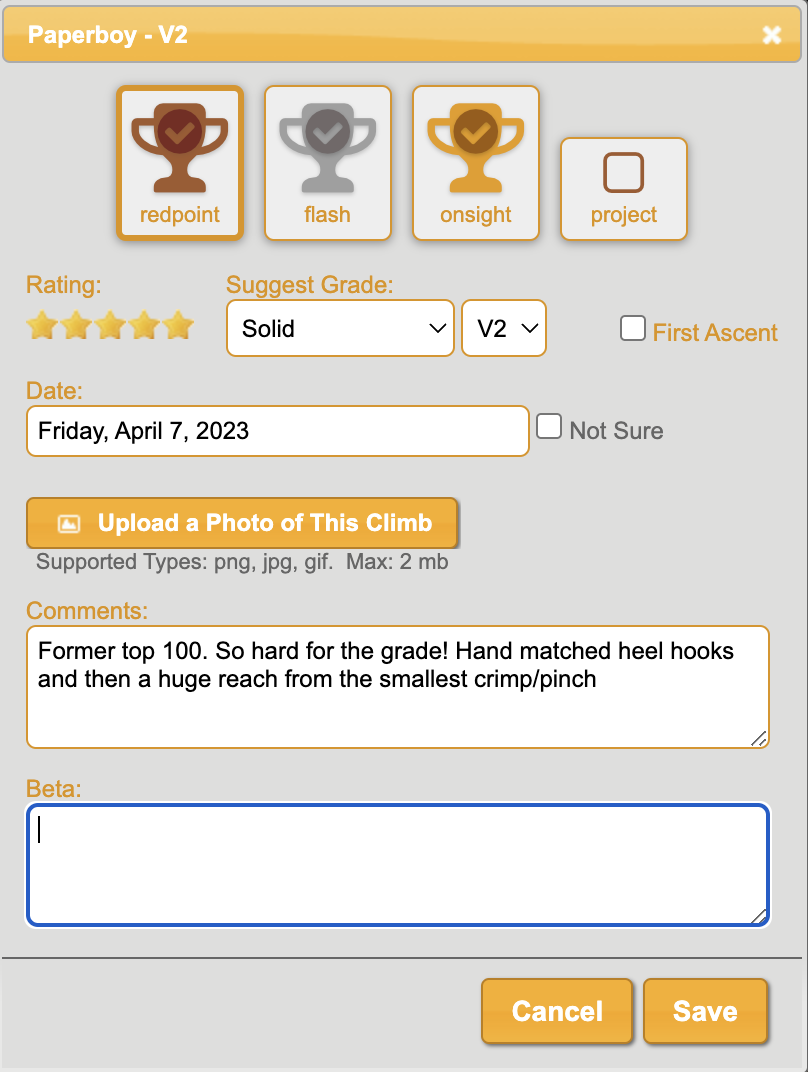
\includegraphics[scale=0.4]{sendage.png}
  \caption{For each send, the boulderer logs the date, any comments and/or "beta" used (the holds, moves or sequence to climb the boulder); they can rate the problem 1-5 stars and give a "feels-like" grade. The date defaults to the current date, so we can expect a few days error in some logged climbs if users do not manually set the actual date the problem was climbed. The default grade is the mean grade of previous logged sends; this biases the user heavily to agree to already proposed grades.}
  \label{fig:sendage}
\end{figure}


\section{Data}

All models were trained on data captured\footnote[2]{March 26, 2023} from the climbing website \href{https://sendage.com}{sendage.com} created and maintained by Jamie Chong, a developer and climber based in Vancouver. It's similar to the larger more well known site \href{https://www.8a.nu/}{8a.nu}, but the climb information is far better curated creating a much cleaner dataset with accurate location data for climbs and practically no duplicates. 

I limited my analysis to boulders, as opposed to sport climbs and trad climbs, because they are more heavily tracked on the site. The most popular boulder problem, Superfly, has nearly 700 "sends" vs 240 ascents of the most popular sport route, Rug Munchers; 45 boulder problems have more logged sends than Rug Munchers. The most popular trad route, Diedre, has only been logged 186 times, despite there being a queue of parties waiting for Diedre every day the weather clears. 

To ensure enough data for boulder problems and boulderers alike, I filtered down to a self-consistent set of problems with at least 5 sends and boulderers that sent at least 5 boulders. For BC, that reduces to 2844 boulder problems, 1069 boulderers that logged 68,336 sends; if I include much of the world, that only increases to 5367 problems, 1428 boulderers with 116,997 sends (the site is mostly used by BC climbers). In BC, each climber has logged 64 problems on average and one has logged 1281 problems; more globally\footnote[3]{Including the West Coast of Canada and the USA and countries with at least a few thousand climbs. To be more consistent, in the next iteration, I will include all regions with a minimum of 1000 climbs.}, they've logged 82 on average (and that same climber has logged 1578 problems over the greater region). BC boulders after filtering under-visited problems have 24 sends on average; more globally, the boulders have 22 sends on average.

Figure \ref{fig:sendage} shows a sendage prompt to log a climb. The mean rating is 3.3 with 74\% rated in BC (3.2 and 72\% more globally); 38\% / 2\% fraction of sends have logged comments or beta in BC (41\% and 1.7\% more globally), respectively. The mean range of assigned grades to a particular problem is less than 1 V grade; the maximum range is 2 V grades\footnote[4]{\href{https://www.99boulders.com/bouldering-grades}{Bouldering grades} in North America follow the "V scale" that was created by John Sherman in the 1980s. A beginner shouldn't be surprised if even V0 feels impossible; there are currently four boulders with the proposed grade V17 and only one of these has seen repeats to confirm the grade.}. The most popular grade logged is V4 with a linear drop up to V11 and a few harder sends up to V14; likewise, there are fewer V0-V3 boulders logged (mostly because many climbers don't log the "easy" problems). 



% Likely to be very detailed if the datasets are new or unfamiliar to the community, or if familiar datasets are being used in new ways.
% Includes prior work on them, statistics, and a collection protocol. 

\section{Model}

The bouldering recommender uses a transformer model with fixed position embeddings. The input included: learned boulder embeddings; learned climber embeddings; logged rating and grade as numerical features; comments or beta if provided as an indicator variable; region one-hot encoded; and elapsed days since the last logged boulder as a numerical feature. 

All training was done on a single NVIDIA RTX 2070 8GB GPU (training time was <1 min; on a CPU it was ~10-100x slower). 

% Flesh out your own approach, perhaps amplifying themes from the `Prior lit' section.

\section{Methods}

The model was trained on BC data and then global data, the latter being less connected. 
The data was split into train, dev and test sets by climber with 85/5/10 splits. This ensured that the user preferences wouldn't leak from the dev and test sets. The full history of each climber was split into all contiguous subsequences of length n=10; for users with fewer than 10 boulders logged, I padded the start of their sequence with MASK tokens. Only the climb token itself is masked in the sequence; all other features are used to prompt the missing climb. This makes the task easier but also more relevant to a bouldering recommender (the climber has a location and grade in mind, and generally wants a 5-star problem).

Simpler models were implemented and compared against: the CBOW model of word2vec \cite{word2vec}, and a 1-2 GRU unit model. The CBOW model doesn't model the sequence at all; the GRU model has no attention. Both models were trained purely on climb embeddings. 

The transformer implementation was adapted from an \href{https://github.com/google/flax/blob/main/examples/nlp_seq/models.py}{example} in the Flax library; this is in JAX. Dropout and layer normalization are both used as in the standard transformer architecture. Softmax cross entropy loss was minimized using the adam optimizer; hyperparameter tuning maximized prediction accuracy. The learning rate has a short warmup period growing to a maximum rate of 10$^{-3}$ and then slowing with a cosine decay down to 10$^{-4}$. Early stopping is used after 10 epochs of no improved accuracy on the validation set.

CBOW has a single dense layer of dimension 128; each GRU unit dimension is 128.

The transformer model was tested with 1-4 heads in 1-2 layers. The attention matrices had dimension 64, as do the dense layers. The climb embedding dimension was tested at 48, 96 and 124; the climber embedding was much smaller, typically between 8 and 16.

% The experimental approach, including descriptions of metrics, baseline models, etc. Details about hyperparameters, optimization choices, etc., are probably best given in appendices, unless they are central to the arguments.

% Explicitly define the metrics, even the common ones (or at least reference them). Be clear about how the data is split for assessment. 


\begin{table}[h]
  \centering
  \begin{tabular}{r | l}
    \textbf{model type} & \textbf{accuracy} \\
    \hline \\
    CBOW & 0.077 \\
    GRU & 0.0846 \\
    Transformer model with features: & \\
    climb embeddings & 0.099 \\
    and other features & 0.24  \\
    and climber embeddings & 0.24 \\
    climber embedding, but no other features & 0.19
    
  \end{tabular}
  \caption{BC results}
  \label{tab:BC}
\end{table}

\begin{table}[h]
  \centering
  \begin{tabular}{r | l}
    \textbf{model type} & \textbf{accuracy} \\
    \hline \\
    CBOW & 0.079 \\
    GRU & 0.085 \\
    Transformer model with features: & \\
    climb embeddings & 0.078 \\
    and other features & 0.23  \\
    and climber embeddings & 0.23 \\
    climber embedding, but no other features & 0.08
    
  \end{tabular}
  \caption{Results for all regions.}
  \label{tab:all}
\end{table}

\section{Results} 

Tables \ref{tab:BC} and \ref{tab:all} show the results of the three models and the transformer model trained on just climb embeddings, or with climber embeddings and/or other features. The three models are indistinguishable (especially considering the minimal hyperparameter tuning each model received). The inclusion of additional features, particularly the unmasked other features to prompt the next climbing token, by far provided the greatest improvement in prediction accuracy. 

For the BC subset, climber embeddings without the extra features improves performance by nearly 10\% and yet the embeddings of the climbers in the held out test set are not trained at all. 

A further clue I have that climber embeddings do help the model is that the training accuracy is higher when they are included while generalization error stays the same: in BC, the training accuracy without climber embeddings is 0.49 with generalization accuracy dropping to 0.24; with the climber embeddings, the training accuracy is 0.57 with the same test error. While this is not evidence of much at all it does push me to try other train/test splits to see how partially trained climber embeddings help on held out recent sequences. 

% A no-nonsense report of what happened.

\section{Analysis} 

The transformer model doesn't come out as a clear winner; the additional user embeddings may not be worth the added complication of cold start for new users. Next item prediction is a hard task given how noisy the logged climb sequences are; that climb embeddings alone reach nearly 10\% accuracy for the more densely connected BC subset is quite astonishing. By adding location and grade, predictions are correct nearly 1 every 4. I cannot even predict the next boulder I will climb with such accuracy.

% Discussion of what the results mean, what they don’t mean, where they can be improved, etc. These sections vary a lot depending on the nature of the paper. (For papers reporting on experiments with multiple datasets, it can be good to repeats Methods/Results/Analysis in separate (sub)sections for each dataset.)

\section{Conclusion} 

Models borrowed from natural language processing adapt well to sequential recommendations. The spaces remain quite different: the number of items and users can be far higher and yet the number of interactions is limited (compare with the wealth of text current language models can train on). The inclusion of other features by concatenating them is simple and proves quite helpful. A better train/test split specific to recommendations should allow for training user embeddings while assuring no leakage of the test data. No overlapping segments of climbs should be shared across splits. 

% Quickly summarize what the paper did, and then chart out possible future directions that anyone might pursue.

\section*{Known Project Limitations}

The most glaring missing piece in this approach is how to train the new user embeddings without have to train or fine-tune the entire model. The easiest approach would be to borrow the embeddings (or average embeddings) of the most similar other climbers. Another approach would be to freeze the climb embeddings and all the other user embeddings and fine-tune the model on the new users for a few iterations. Also, it would be interesting the try a different train/dev/test split to compare users with trained embeddings with held-out most recent sequences. 

The metric used, accuracy, is not ideal for a recommender. For the next iteration, I will switch to recall or mean reciprocal rank (I just didn't have time). A ranking loss should be compared to the softmax cross entropy. A more thorough hyperparameter search would almost certainly improve performance. 

The data supports longer sequences, but my system wasn't stable enough to train them. My ablation tests should more finely examine the addition of various features.

The Transformers4Rec analysis showed that MLM performed best, and it's only a small change to my pipeline; also, they showed that numerical features were easier to learn from binned and one-hot encoded. Masking longer contiguous sections to enable such recommendations would be more useful for the climber targeting a specific project but lacking the skills to complete it. The chain of boulder problems recommended, if completed, should allow the climber to gain these skills.  

The time elapsed should not be a separate numerical feature, but rather it should be used to enforce sequence order in the position embeddings. This should naturally model the climbs as a sequence of sessions. 

Finally, it would be fascinating to add text embeddings of logged comments and beta. I expect the model can learn from, e.g. "Intimidating landing but secure moves.", "High sit start on jug rail, mantle exit. Reachy." or "Definitely suited me, all of the difficulty in the 1st move. Psyched!"

The recommender should be tested in another domain. Early readers have a similar skill progression. Modelling the sequence of books read by young readers would be an interesting application of this approach.

% For this section, imagine that your reader is a well-intentioned NLP practitioner who is seeking to make use of your data, models, or findings as part of a separate scholarly project, deployed system, or some other kind of real-world intervention. What should such a person know about your work? Especially important here are limitations and biases that might affect this person, their findings, their experiment participants, or the users of their product or service. The idea is that what you say here will be taken into consideration but this well-intentioned user, leading to better outcomes for everyone.

\section*{Authorship Statement}

I worked on this project solo including the literature review, the iterative implementation and experimentation, result gathering and final writing up. I had many fruitful conversations with Alistair Fraser, also taking the course, and Michael Nathe about my design choices and result analysis. 

\bibliography{project}

% \appendix

% \section{Example Appendix}\label{sec:appendix}

% This is an appendix.

\end{document}
